%------------------------------------------%
% Cannabis Data Science
% Saturday Morning Statistics
% Date: 3/12/2022
%------------------------------------------%
\documentclass[xcolor={dvipsnames}]{beamer}
\hypersetup{pdfpagemode = FullScreen}
\mode<presentation>{
  \usetheme{Boadilla}
  \usecolortheme{orchid}
  \usefonttheme{default}
  \setbeamertemplate{navigation symbols}{}
  \setbeamertemplate{caption}[numbered]
}
\setbeamersize{
  text margin left = 0.5in,
  text margin right = 0.5in
}

%------------------------------------------%
% Title
%------------------------------------------%
\author{Cannabis Data Science}
\title[\textbf{Saturday Morning Statistics \#15}]{}
\institute[]{\Large Saturday Morning Statistics \#15}
\date{March \nth{12}, 2022}

%------------------------------------------%
% Packages
%------------------------------------------%
\usepackage[english]{babel}
\usepackage[utf8x]{inputenc}
\usepackage{tikz}
\usepackage{xparse}

%------------------------------------------%
% Colors
%------------------------------------------%
\definecolor{Green}{RGB}{34, 153, 84}
\definecolor{LightGreen}{RGB}{218, 247, 166}
\definecolor{DarkGreen}{RGB}{2, 48, 32}
\definecolor{Orange}{RGB}{255, 87, 51}
\definecolor{DarkOrange}{RGB}{199, 0, 57}
\definecolor{Yellow}{RGB}{255, 195, 0}

%------------------------------------------%
% Theme
%------------------------------------------%
\setbeamercolor*{palette primary}{bg=LightGreen, fg=DarkGreen}
\setbeamercolor*{palette secondary}{bg=LightGreen, fg=DarkGreen}
\setbeamercolor*{palette tertiary}{bg=LightGreen, fg=DarkGreen}

%------------------------------------------%
% Packages
%------------------------------------------%
\usepackage{amsmath}
\renewcommand*\footnoterule{} % No separating line on footnote.
\usepackage{mathtools} % For annotating equations.
\usepackage{hhline} % for double bars.
\usepackage[super]{nth} % For formatting 1st, 2nd, 3rd, etc.
\usepackage{graphicx, caption, subcaption}
\usepackage{setspace}

%------------------------------------------%
% Commands
%------------------------------------------%

% Top space.
\newcommand\T{\rule{0pt}{2.5ex}}

% Bottom space.
\newcommand\B{\rule[-1.25ex]{0pt}{0pt}}

% Blocks.
\newenvironment<>{Block}[2][.9\textwidth]
  {\setlength{\textwidth}{#1}
  \begin{actionenv}#3
    \def\insertblocktitle{#2}\par
    \usebeamertemplate{block begin}}
  {\par\usebeamertemplate{block end}
  \end{actionenv}}

% Balls.
\defbeamertemplate{enumerate item}{largeball}
{\begin{pgfpicture}{-1ex}{-0.65ex}{1.5ex}{1.5ex}
\usebeamercolor[fg]{item projected}
{\pgftransformscale{2.5}\pgftext{\Large\pgfuseshading{bigsphere}}}
{\pgftransformshift{\pgfpoint{0pt}{0.5pt}}
\pgftext{\usebeamerfont*{item projected}\small\insertenumlabel}}
\end{pgfpicture}}

% Fancy arrows.
\NewDocumentCommand\UpArrow{O{2.0ex} O{black}}{%
   \mathrel{\tikz[baseline] \draw [->, line width=0.5pt, #2] (0,0) -- ++(0,#1);}} % Fancy up-arrow.
\NewDocumentCommand\DownArrow{O{2.0ex} O{black}}{%
   \mathrel{\tikz[baseline] \draw [<-, line width=0.5pt, #2] (0,0) -- ++(0,#1);}} % Fancy down-arrow.

% Equations with numbers on the left.
\makeatletter
\newcommand{\LeftEqNo}{\let\veqno\@@leqno}
\makeatother

%------------------------------------------%
% Presentation
%------------------------------------------%
\begin{document}

%------------------------------------------%
% Title Page
%------------------------------------------%
\begin{frame}{}
  
\includegraphics[scale=0.33]{images/logo.pdf}
  \vspace*{-2\baselineskip}
  \titlepage
\end{frame}

%------------------------------------------%
% Statistical History
%------------------------------------------%
\section{Background}
\begin{frame}{A Brief Background}

\begin{minipage}{0.35\textwidth}
\begin{figure}
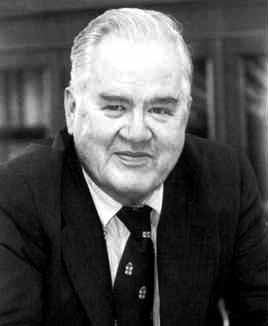
\includegraphics[width=\textwidth]{images/john-tukey.jpg}
\caption*{\footnotesize John Tukey (1915 - 2000)\\Professor of Statistics at Princeton University}
\end{figure}
\end{minipage}\hspace{0.05\textwidth}%
\begin{minipage}{0.55\textwidth}

\vspace{-1\baselineskip}
{\bfseries John Tukey}
\vspace{0.25\baselineskip}

\begin{itemize}

\item Created the \underline{box plot}.

\item Coined the term {``\itshape bit''}.

\item First published use of the word {\bfseries software}.

\item Creator of the \underline{median--median line} (an alternative to the linear regression).

\item Creator of the \underline{trimean} measure of central tendency

\vspace*{-1\baselineskip}
$$
TM = \frac{Q_1 + 2Q_2 + Q3}{4}
$$

\end{itemize}
\end{minipage}

\begin{itemize}

\vspace*{0.5\baselineskip}
\item {\bfseries Exploratory data analysis} vs. {\bfseries confirmatory data analysis}.

\item The data should determine the methodology used.

\end{itemize}


\end{frame}


%------------------------------------------%
% Introduction
%------------------------------------------%
\section{Introduction}
\begin{frame}{Survival Analysis}

\vspace*{2\baselineskip}

%% TODO: Pharmacology
%% https://en.wikipedia.org/wiki/Pharmacology

\vspace{-2\baselineskip}

% Question of the day
\begin{center}
\begin{minipage}{.9\linewidth}
\begin{Block}{Question of the day.}

\vspace{.5\baselineskip}
\begin{itemize}
\item  {\bfseries Survival analysis} has largely been pioneered by medical researchers to study \underline{lifetimes}. Can we apply survival analysis to study the question: what is the natural \underline{lifetime} of a retailer or producer in in the cannabis industry?

\end{itemize}

\vspace{.5\baselineskip}

\end{Block}
\end{minipage}
\end{center}

\vspace{1\baselineskip}

{\bfseries Survival function}: $S(t) = P(T > t).$

\vspace{.5\baselineskip}

{\bfseries Hazard function}: $\lambda(t) = -\frac{S^\prime(t)}{S(t)}.$

\end{frame}


% TODO: Introduce survival function


% TODO: Introduce hazard rate


%------------------------------------------%
% History
%------------------------------------------%

\begin{frame}{}

{\bfseries Poisson regressions} have historically been used to approximate {\bfseries proportional hazards models}.

\vspace{.75\baselineskip}
\begin{itemize}

\item Calculation is \underline{quicker}.

\vspace{.75\baselineskip}

\item Originally important when computers were \underline{slower}.

\vspace{.75\baselineskip}

\item Also helpful with \underline{large data} sets or \underline{complex models}.

\end{itemize}

\vspace{.75\baselineskip}
\begin{center}
\begin{minipage}{0.75\textwidth}
\itshape ``we do not assume [the Poisson model] is true, but simply use it as a device for deriving the likelihood.''\\
\vspace*{-1.5\baselineskip}
\begin{flushright}
{\footnotesize -- Laird and Olivier (1981)}
\end{flushright}
\end{minipage}
\end{center}

\end{frame}

%------------------------------------------%
% Kaplan–Meier estimator
%------------------------------------------%
\begin{frame}{}

\vspace{1\baselineskip}
{\large \textbf{Kaplan--Meier Estimator}}\vspace{0.75\baselineskip}\\

\begin{itemize}

\item Used to estimate \underline{survival functions}.

\vspace{0.75\baselineskip}

\item One of the most frequently used methods of survival analysis.

\vspace{0.75\baselineskip}

\item The estimator is given by

$$
\hat{S}(t) = \sum_{t_i=0}^{t_i\leq t}\left(1 - \frac{d_i}{n_i}\right)
$$

where

\vspace{0.25\baselineskip}
\begin{itemize}
\item $t_i$ is exposure time,
\vspace{0.25\baselineskip}
\item $d_i$ is the number of events at time $t_i$,
\vspace{0.25\baselineskip}
\item $n_i$ is the number of individuals known to have survived up to time $t_i$.
\end{itemize}

\end{itemize}

\end{frame}


% TODO: Figure of KM Plot.

%------------------------------------------%
% Nelson–Aalen estimator
%------------------------------------------%
\begin{frame}{}

\vspace{1\baselineskip}
{\large \textbf{Nelson--Aalen Estimator}}\vspace{0.75\baselineskip}\\

\begin{itemize}

\item An estimator of the \underline{cumulative hazard rate function} given {\itshape censored data} or {\itshape incomplete data}.

\vspace{0.75\baselineskip}

\item The estimator is given by
$$
\hat{H}(t) = \sum_{t_i=0}^{t_i\leq t} \frac{d_i}{n_i}
$$

where

\vspace{0.25\baselineskip}
\begin{itemize}
\item $t_i$ is exposure time,
\vspace{0.25\baselineskip}
\item $d_i$the number of events at time $t_i$,
\vspace{0.25\baselineskip}
\item $n_i$ is the number of individuals known to have survived up to time $t_i$.
\end{itemize}

\end{itemize}



\end{frame}


%------------------------------------------%
% Cox's proportional hazards model
%------------------------------------------%
\begin{frame}{}

\vspace{1\baselineskip}
{\large \textbf{Cox's Proportional Hazards Model}}\vspace{0.75\baselineskip}\\

Given covariates, $x$, and parameters, $\beta$, the hazard rate is modeled as

$$
\lambda(t) = \lambda_0(t)\text{exp}(x\beta),
$$

where $\lambda_0(t)$ is the baseline hazard.

\vspace{1\baselineskip}

A couple of important assumptions:

\vspace{0.75\baselineskip}

\begin{itemize}

\item The baseline hazard, $\lambda_0(t)$, is assumed to be independent of the covariate, $x$.

\vspace{0.75\baselineskip}

\item The matrix of covariate, $x$, should not include a constant term.

\end{itemize}

\end{frame}


%------------------------------------------%
% Poisson regressions to approximate proportional hazards models
%------------------------------------------%
\begin{frame}{}

\vspace{1\baselineskip}
{\large \textbf{Poisson regressions to approximate proportional hazards models}}\vspace{0.75\baselineskip}\\


If you treat the event indicators, $d_{ij}$, as if they were independent \underline{Poisson-distributed} observations with means

$$
\mu_{ij} = t_{ij}\lambda_{ij}
$$

where $t_{ij}$ is the exposure time and $\lambda_{ij}$ is the hazard for individual $i$ in interval $j$, then taking the log yields a \underline{Poisson log-linear model}

$$\text{log}\mu_{ij} = \text{log}t_{ij} + \alpha_j + x_i^\prime \beta.$$

\end{frame}


%------------------------------------------%
% Time-varying Covariates
%------------------------------------------%
\begin{frame}{}

\vspace{1\baselineskip}
{\large \textbf{Hazards Model with Time-varying Covariates}}\vspace{0.75\baselineskip}\\

Adding \underline{time-varying covariates} to the hazards model yields

$$\text{log}\lambda_{ij} = \alpha_j + \beta x_{ij},$$

where $x_{ij}$ are the values of the covariates of individual $i$ in interval $j$.

\end{frame}



%------------------------------------------%
% Time-dependent Effects
%------------------------------------------%
\begin{frame}{}

\vspace{1\baselineskip}
{\large \textbf{Hazards Model with Time-dependent Effects}}\vspace{0.75\baselineskip}\\

Adding \underline{time-dependent covariates} to the hazards model yields

$$\text{log}\lambda_{ij} = \alpha_j + \beta_j x_{ij},$$

where $\beta_j$ is the effect of the hazard during interval $j$.


\vspace{1\baselineskip}

Assumptions:


\vspace{0.75\baselineskip}
\begin{itemize}

\item Effects vary only at interval boundaries.

\end{itemize}

\end{frame}


%------------------------------------------%
% Cox's proportional hazards model - Bayesian inference
%------------------------------------------%
\begin{frame}{}

\vspace{1\baselineskip}
{\large \textbf{Bayesian Inference of Hazards Model}}\vspace{0.75\baselineskip}\\

\begin{enumerate}

\item First, you specify your priors for the parameters

\vspace*{-1.25\baselineskip}
\begin{align*}
\beta &\sim \mathcal{N}(\mu_\beta, \sigma_\beta^2) \\
\sigma_\beta &\sim \mathcal{U}(a, b) \\
\lambda_j &\sim \Gamma(\alpha, \beta)
\end{align*}

with hyperparameters $\mu_\beta$, $a$, $b$, $\alpha$, and $\beta$.

\vspace{0.75\baselineskip}

\item Second, you simulate draws from the posterior distributions.

\vspace{0.75\baselineskip}

\item Finally, you analyze and interpret your Bayesian estimates.

\end{enumerate}


\end{frame}


%------------------------------------------%
% 
%------------------------------------------%
%\begin{frame}{}
%
%\vspace{1\baselineskip}
%{\large \textbf{}}\vspace{0.75\baselineskip}\\
%
%$$d_{ij} = $$
%
%\end{frame}


%------------------------------------------%
% Takeaway
%------------------------------------------%
\section{Takeaway}
\begin{frame}{}

\begin{center}
\begin{minipage}{3.85in}

% Thank you.
\begin{center}

\includegraphics[width=.25in]{images/prayer.png} {\Large \textbf{Thank you for coming.}}\\
\end{center}
\vspace*{0.5\baselineskip}

% Re-cap the lesson of the week.
\begin{center}
\begin{minipage}{\linewidth}
\begin{Block}{Lessons of the Day}

\vspace{0.5\baselineskip}

\begin{itemize}

\item Borrowing from other fields is fruitful.

\vspace{0.5\baselineskip}

\item Having the right tools (models) for the data at hand is critical.

\vspace{0.5\baselineskip}

\item {\bfseries Survive, then thrive} if you are a cannabis producer or retailer.

\vspace{0.5\baselineskip}

\end{itemize}

\end{Block}
\end{minipage}
\end{center}

\vspace*{2\baselineskip}

\end{minipage}
\end{center}

\end{frame}


%------------------------------------------%
% Fin.
%------------------------------------------%
\end{document}
